\subsection{BERT}
\label{subsec:BERT_results}
To fine-tune our two pre-trained BERT models, Italian BERT and AlBERTo, we carried out the steps described in \ref{subsec:BERT_methods}. We then proceeded to test both models against our two test sets. The main metrics from the final classification reports are presented in Tables \ref{tab:classification_report_bert_base_tweets},\ref{tab:classification_report_bert_base_news},\ref{tab:classification_report_alberto_tweets} and \ref{tab:classification_report_alberto_news}.

\begin{table}[h]
    \centering
    \small
    \begin{tabular}{lcccc}
        \toprule
        & \textbf{Precision} & \textbf{Recall} & \textbf{F1-Score} \\
        \midrule
        0 & 0.7796 & 0.7613 & 0.7703 \\
        1 & 0.7598 & 0.7781 & 0.7689 \\
        \midrule
        \textbf{accuracy} & & & 0.7696 \\
        \textbf{macro Avg F1} &  &  & 0.7696 \\
        \bottomrule
    \end{tabular}
    \caption{Italian BERT classification report for Tweets.}
    \label{tab:classification_report_bert_base_tweets}
\end{table}

\begin{table}[h]
    \centering
    \small
    \begin{tabular}{lccc}
        \toprule
        & \textbf{precision} & \textbf{recall} & \textbf{f1-score} \\
        \midrule
        0 & 0.7290 & 0.9530 & 0.8261 \\
        1 & 0.8193 & 0.3757 & 0.5152 \\
        \midrule
        \textbf{accuracy} & & & 0.7440 \\
        \textbf{macro avg F1} & & & 0.6706 \\
        \bottomrule
    \end{tabular}
    \caption{Italian BERT classification report for News Headlines.}
    \label{tab:classification_report_bert_base_news}
\end{table}

% Requires: \usepackage{graphicx}
\begin{table}[h]
    \centering
    \small
    \begin{tabular}{lccc}
        \toprule
        & \textbf{precision} & \textbf{recall} & \textbf{f1-score} \\
        \midrule
        0 & 0.7805 & 0.7379 & 0.7586 \\
        1 & 0.7443 & 0.7862 & 0.7647 \\
        \midrule
        \textbf{accuracy} & & & 0.7617 \\
        \textbf{macro avg F1} & & & 0.7616 \\
        \bottomrule
    \end{tabular}
    \caption{AlBERTo classification report for Tweets.}
    \label{tab:classification_report_alberto_tweets}
\end{table}

\begin{table}[h]
    \centering
    \small
    \begin{tabular}{lccc}
        \toprule
     & \textbf{precision} & \textbf{recall} & \textbf{f1-score} \\
        \midrule
        \textbf{0}          & 0.7423  & 0.9028 & 0.8147  \\
        \textbf{1}          & 0.7232  & 0.4475 & 0.5529  \\
        \midrule
        \textbf{accuracy}   &         &        & 0.7380  \\
        \textbf{macro avg F1}  &   &  & 0.6838  \\
        \bottomrule
    \end{tabular}
    \caption{AlBERTo classification report for News headlines.}
    \label{tab:classification_report_alberto_news}
\end{table}

Both models had stable performances in the in-domain task, with the Italian BERT performing slightly better than the AlBERTo model, and both saw a significant decrease in performance for the cross-domain task, especially Italian BERT (macro F1: from 0.7696 to 0.6706). This is due to the recall dropping significantly for class 1 (Italian BERT: 0.9530 for class 0 and 0.3757 for class 1; AlBERTo: 0.9028 for class 0 and 0.4475 for class 1): once again, it proves difficult for the models to detect hate speech in news headlines.

It is worth mentioning that even after reducing the number of epochs to two, the validation loss still shows a slight upward trend for both models \ref{fig:bert_base_losses}\ref{fig:alberto_losses}. It would be beneficial to delve deeper into hyperparameter tuning and regularization techniques to see how much the performances of the models could improve.

\begin{figure}
    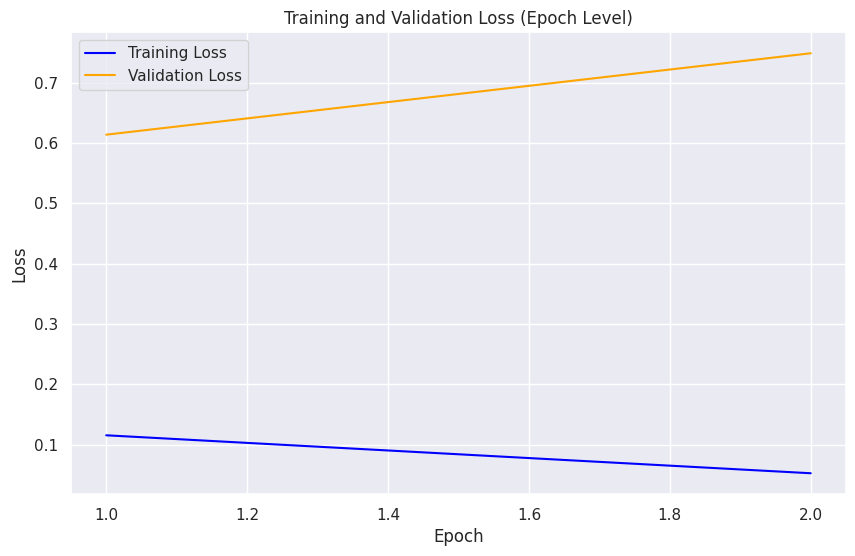
\includegraphics[width=\columnwidth]{../../results/images/bert_base_losses_2epochs.png}
    \caption{Italian BERT Training and Validation Loss trend (LR = 2e-5, Epochs = 2).}
    \label{fig:bert_base_losses}
\end{figure}

\begin{figure}
    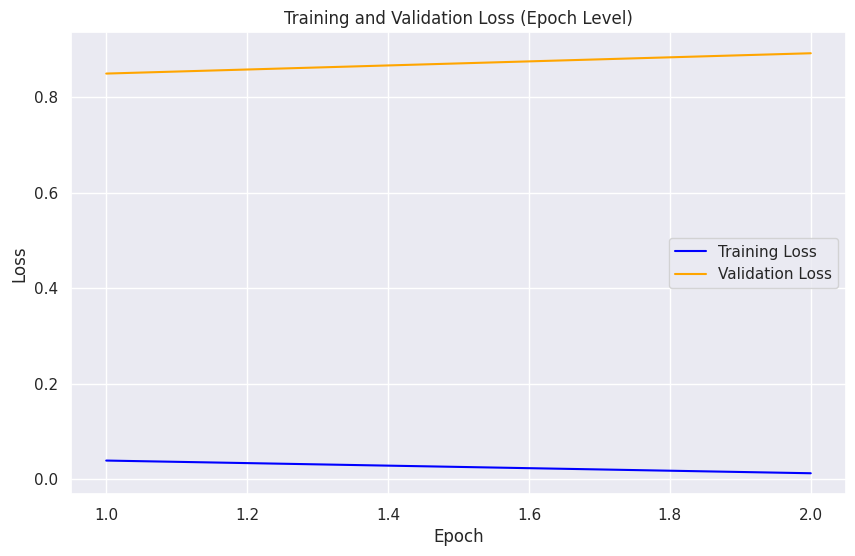
\includegraphics[width=\columnwidth]{../../results/images/alberto_losses_2epochs.png}
    \caption{AlBERTo Training and Validation Loss trend (LR = 2e-5, Epochs = 2).}
    \label{fig:alberto_losses}
\end{figure}